\begin{figure}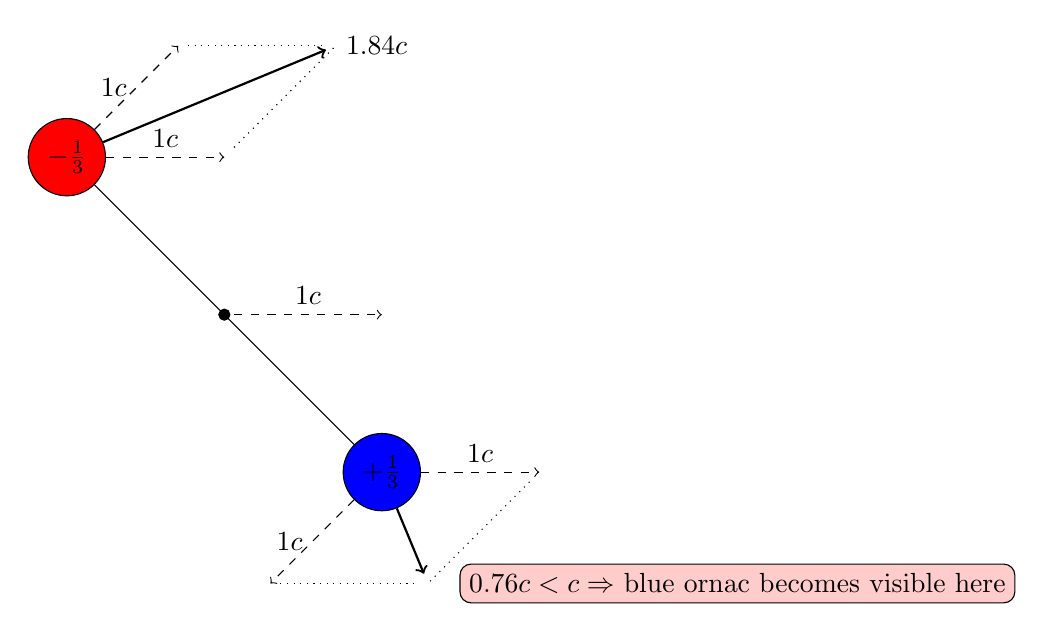
\begin{tikzpicture}[scale=1, rotate=0]


% photon diagonal with speed vectors



\path 
(0,4) node[circle,draw, fill=red](red) {$-\frac{1}{3}$}
(4,0) node[circle,draw, fill=blue](blue) {$+\frac{1}{3}$};
\draw[black] (red) -- (blue)          node[pos=0.5](center){};
\filldraw
 (center) circle (2pt);
\draw[->,dashed, black] (center) -- node[above] { $1c$} ++(2,0) node [anchor=west]{};

%% Arrows indicating the speed components from blue
\draw[->, black, dashed] (blue) -- node[above] { $1c$} ++(2,0) node [](west){};
\draw[->, black, dashed] (blue) -- node[left] { $1c$} ++(225:2) node [](south){};
\draw[ black, dotted] (west) -- ++(225:2) node [](southwest){};
\draw[ black, dotted] (south) -- (southwest) node []{};
\draw[->, black, thick] (blue) --  (southwest) node (under_c) {};
\path
(under_c)+(0.4,0)node [fill=red!20,draw, rounded corners, right]
{ $0.76c < c \Rightarrow$ blue ornac becomes visible here};

%% Arrows indicating the speed components from red
\draw[->, black, dashed] (red) -- node[above] { $1c$} ++(2,0) node [](redwest){};
\draw[->, black, dashed] (red) -- node[left] { $1c$} ++(45:2) node [](redsouth){};
\draw[ black, dotted] (redwest) -- ++(45:2) node [](redsouthwest){};
\draw[ black, dotted] (redsouth) -- (redsouthwest) node []{};
\draw[->, black, thick] (red) --  (redsouthwest) node [below, right] { $1.84c$};

\end{tikzpicture}\caption{Photon diagonal with speed vectors
\label{fig:photon-diagonal}}
\end{figure}
